\documentclass[fleqn,10pt,doc,onecolumn]{SelfArx}%article} % Document font size and equations flushed left

\usepackage{float}
\usepackage{graphicx}
\usepackage{caption}
\usepackage[hyphens]{url}
\usepackage{hyperref}
\usepackage{xcolor}
\usepackage{amsmath}
\usepackage[switch,pagewise]{lineno}
\linenumbers

\graphicspath{{figures/}}
\setlength{\abovecaptionskip}{15pt plus 3pt minus 2pt}

\newcommand{\beginsupplement}{%
        \setcounter{table}{0}
        \renewcommand{\thetable}{S\arabic{table}}%
        \setcounter{figure}{0}
        \renewcommand{\thefigure}{S\arabic{figure}}%
     }

\definecolor{color1}{RGB}{0,0,90} % Color of the article title and sections
\definecolor{color2}{RGB}{200,200,200} % Color of the boxes behind the abstract and headings
\definecolor{color3}{RGB}{5,5,5} % Color of the boxes behind the abstract and headings

\JournalInfo{.} % Journal information ``Journal, Vol. XXI, No. 1, 1-5, 2015''
\Archive{ } % Additional notes (e.g. copyright, DOI, review/research article)

\PaperTitle{A Bioinformatician, Computer Scientist, and Geneticist lead bioinformatic tool development - which one is better?}

\Authors{Paul P. Gardner\textsuperscript{1}*}
  
\affiliation{\textsuperscript{1}\textit{Department of Biochemistry, University of Otago, Dunedin, New Zealand.}} % Author affiliation
\affiliation{*\textbf{Corresponding author}: paul.gardner@otago.ac.nz} % Corresponding author


\Keywords{
Bioinformatics,
Software Tool Development, 
Interdisciplinary Research, 
Departmental Affiliation, 
Software Accuracy, 
Medical Informatics, 
Academic Expertise, 
Benchmarking,
Computational Biology
} % Keywords - if you don't want any simply remove all the text between the curly brackets
\newcommand{\keywordname}{Keywords} % Defines the keywords heading name

%----------------------------------------------------------------------------------------
%       ABSTRACT
%----------------------------------------------------------------------------------------
\Abstract{The development of accurate bioinformatic software tools is
  crucial for the effective analysis of complex biological data. This
  study examines the relationship between the academic department
  affiliations of authors and the accuracy of the bioinformatic tools
  they develop. By analyzing a corpus of previously benchmarked
  bioinformatic software tools, we mapped bioinformatic tools to the
  academic fields of the corresponding authors and evaluated tool
  accuracy by field. Our results suggest that ``Medical Informatics''
  outperforms all other fields in bioinformatic software accuracy,
  with a mean proportion of wins in accuracy rankings exceeding the
  null expectation. In contrast, tools developed by authors affiliated
  with "Bioinformatics" and "Engineering" fields tend to be less
  accurate. However, after correcting for multiple testing, no
  result is statistically significant ($p>0.05$). Our findings
  reveal no strong association between academic field and
  bioinformatic software accuracy. These findings suggest that the
  development of interdisciplinary software applications can be
  effectively undertaken by any department with sufficient resources
  and training.}

\begin{document}

\flushbottom % Makes all text pages the same height
\maketitle % Print the title and abstract box
%\tableofcontents % Print the contents section

\thispagestyle{empty} % Removes page numbering from the first page

\section*{Background}

Departmental divisions in academia signify research expertise,
influence hiring decisions, and impact access to funding, publishing
opportunities, and student training
\cite{bourke1998institutions,ben2016s}. However, interdisciplinary
fields such as bioinformatics blur traditional boundaries by
integrating data and methods from biology, computer science, and
mathematics to address complex research challenges
\cite{Ouzounis:2003,Eddy:2005,hogeweg2011roots}.

Bioinformatics has become essential to modern biological research,
facilitating evolutionary, structural, and functional analyses of
genomic, transcriptomic, and proteomic data
\cite{clement2018data,gauthier2019brief}. The development of accurate and
scalable bioinformatic tools is critical for interpreting such large
datasets. Which requires both biological insight and advanced
computational skills to build algorithms. The advent of
high-throughput technologies has driven the growth of bioinformatics,
leading to the establishment of specialized groups within biology,
computer science, and engineering faculties, each contributing to the
field’s expansion
\cite{hogeweg2011roots,gauthier2019brief}.

The contributions of ``domain experts'' to bioinformatics from the
biological and health sciences, such as genetics and molecular biology
are essential as they ensure software tools are relevant and accurate.
However, domain experts may lack the advanced computational expertise
needed to develop sophisticated software. In contrast, fields like
mathematics, engineering, and computational sciences — referred to
here as ``development experts'' — offer expertise in algorithm
development, mathematical modeling, statistics, and software
engineering, essential for creating efficient and scalable
bioinformatic tools.

It is possible that departmental differences may influence
bioinformatic tool development by reflecting the distinct expertise,
resources, and perspectives offered by different academic
fields. Development experts excel in computational efficiency, while
domain experts provide essential biological insights. Therefore, the
success of a tool may depend on the integration of diverse
skills rather than on the specific departmental affiliation of its
developers. 

The primary objective of this study is to examine whether the academic
department affiliation of a corresponding author has a discernible
outcome on the accuracy (i.e. correctness of predictions) of the
bioinformatic tools they develop. Specifically, we aim to determine
whether tools created by authors from domain-expert,
development-expert of interdisciplinary fields differ in accuracy. To
address this, we analyzed a benchmarked corpus of bioinformatic
software tools and evaluated their accuracy based on the developers'
academic affiliations.


\begin{figure*}[t!]
  \centering
  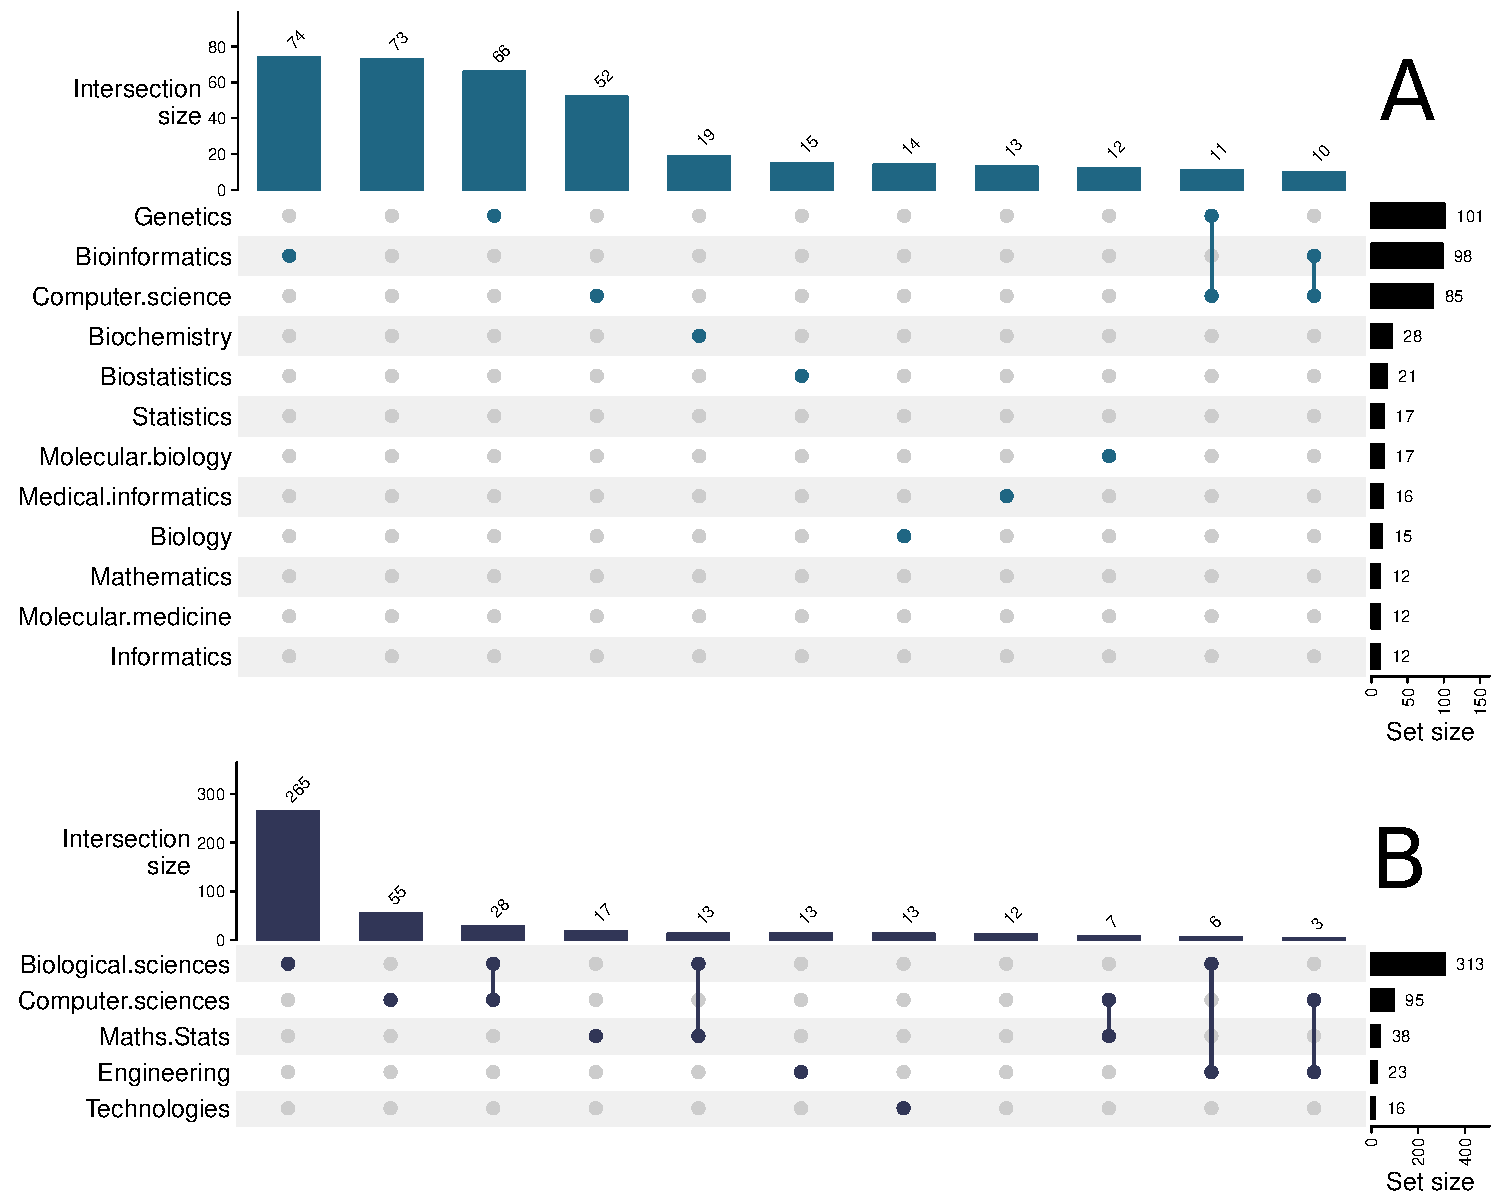
\includegraphics[width=0.75\textwidth]{upset-plots.pdf}
  \caption{ The number and intersection of general (\textbf{A}) or
  specific (\textbf{B}) fields that have contributed to bioinformatic
  software tools included in recent benchmark studies.  The number and
  intersection of specific fields.  }
\label{fig:fig1}
\end{figure*}



%%%%%%%%%%%%%%%%%%%%%%%%%%%%%%%%%%%%%%%%%%%%%%%%%%%%%%%%%%%%%%%%%%%%%%
\section*{Results}

We explored the relationship between the accuracy of bioinformatic
software tools and the academic fields of their developers. Using a
previously published corpus of benchmarked accuracy rankings
\cite{gardner2024}, we mapped corresponding authors' addresses to
standardized ``fields of study'' \cite{fields2014} and grouped them into
broader categories.

%
Figure~\ref{fig:fig1} shows the number of tools for the general and
specific fields ($N\ge 10$). Most bioinformatic tools were developed
by authors affiliated with Genetics, Bioinformatics, Computer Science,
or similar departments. Among the general fields, Biological Sciences
produced the most software tools, followed by Computer Sciences.


\begin{figure*}[ht!]
\begin{center}
  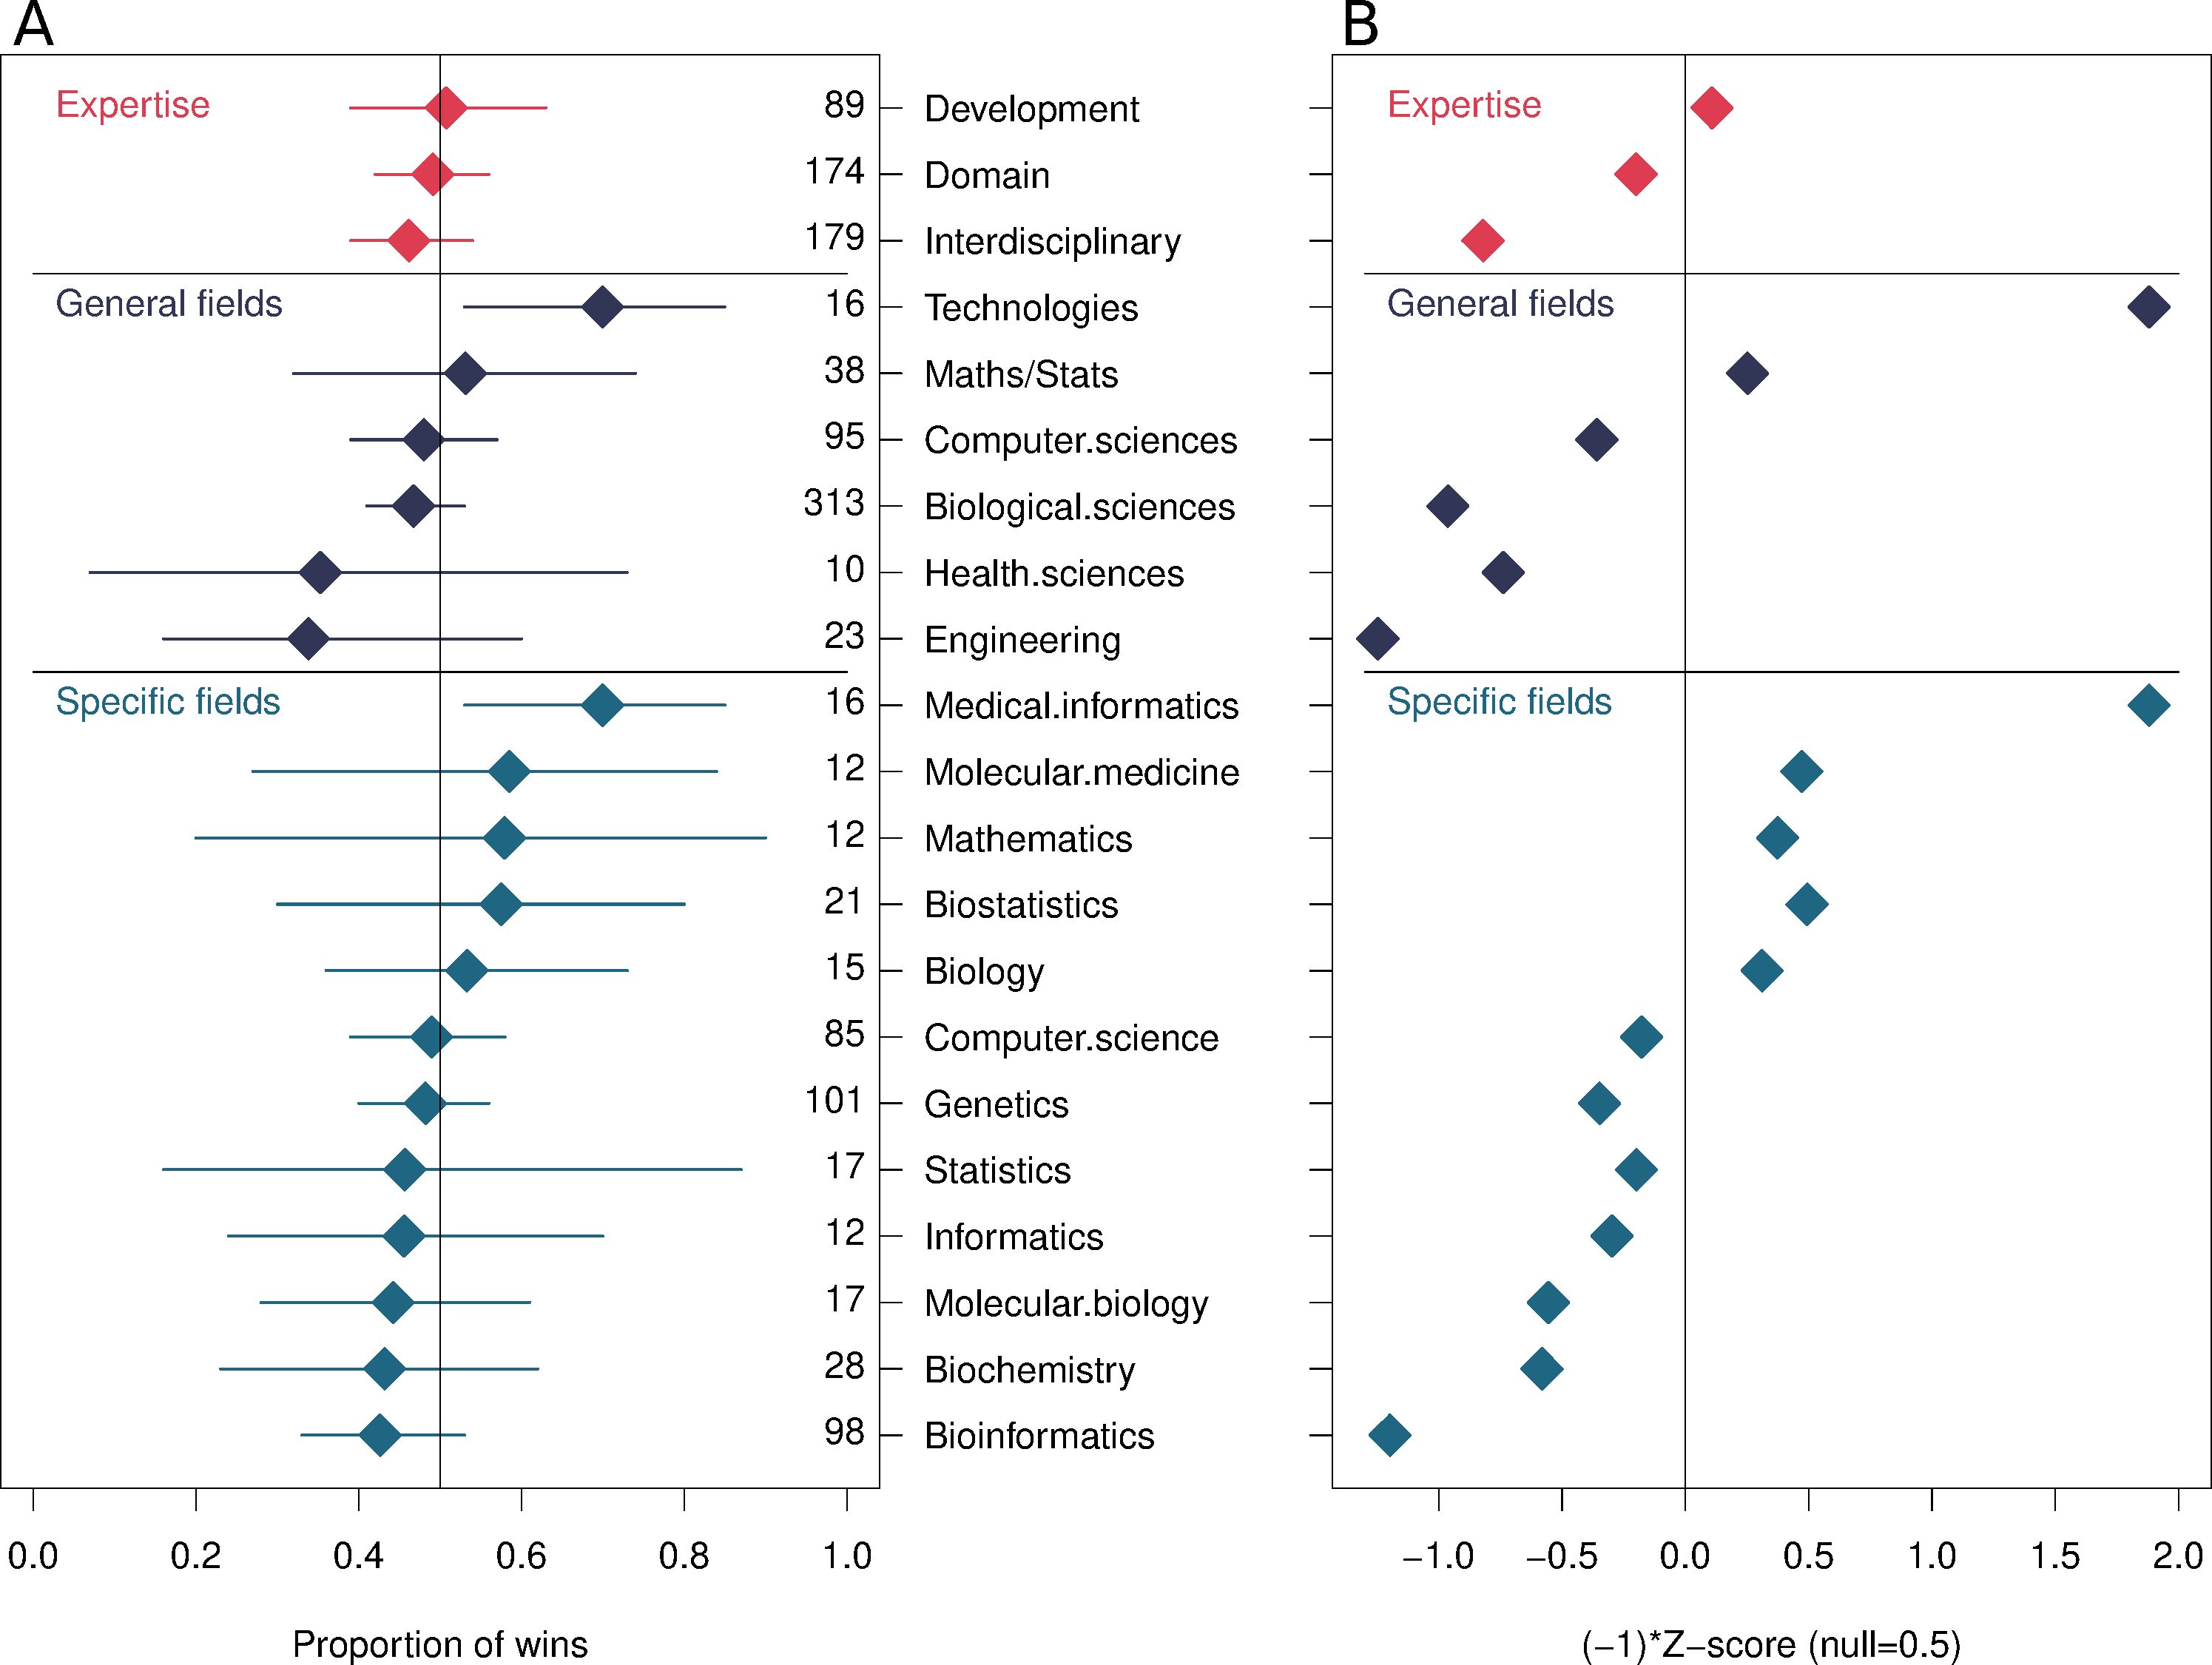
\includegraphics[width=0.65\textwidth]{forest-z-Plot.pdf}
\end{center}
\caption{(\textbf{A}) A forest plot, illustrating the mean and 95\%
  confidence intervals of the proportion of times software tools
  published by a given field ``win'' in pairwise
  comparisons. Confidence intervals and the mean was determined using
  a bootstrapping procedure. Within each field the entries have been
  sorted by the mean number of wins. The sample size for each field is
  indicated by the column of numbers on the right of the figure.
  (\textbf{B}) A Z-score was computed for each distribution of
  bootstrap samples for each field. The expected proportion of wins
  for randomly selected groups of tools was used as ``$x$''
  (i.e. null=0.5).}
\label{fig:fig2}
\end{figure*}


We ranked fields based on the mean proportion of ``wins'' (i.e., for field '1' when its tool
'A' outperforms tool 'B' in benchmark 'X') and calculated Z-scores
to compare them against random expectations (i.e., $wins = 0.5$). A
higher proportion of wins and lower $(-1) * Z-score$ indicate better
overall accuracy.

``Medical Informatics'', a branch of ``Technologies'', outperformed
other fields, with a mean win proportion of 0.70 (95\% CI:
$0.53-0.85$) and a Z-score of $-1.88$. However, P = 0.29 after
multiple testing correction). Notably, this category includes five
different parameter options for the MAFFT sequence alignment tool
\cite{katoh2008recent}, and a further four separate corresponding
authors that list either the Department or Center of Biomedical
Informatics, Harvard Medical School as their affiliation
\cite{kim2010rsw,yang2013diverse,kharchenko2014bayesian,ruan2020fast}. This
and some other redundancies leaves just eight departments
representing the medical informatics field here.


In contrast, ``Bioinformatics'' has the lowest rank, with a mean win
proportion of 0.43 (95\% CI: $0.33-0.53$) and a Z-score of $1.20$ (P =
0.46 after correction). Similarly, ``Engineering'' ranked low, with a
win proportion of 0.34 (95\% CI: $0.16-0.60$) and a Z-score of $1.25$.

Other fields showed confidence intervals that included the null value
of 0.5, with modest Z-scores ranging from -0.49 to 0.96, and P-values
greater than 0.05.

When grouped by expertise type—software development experts,
biological domain experts, or interdisciplinary experts—all categories
had similar win proportions (0.51, 0.49, and 0.46,
respectively). Interdisciplinary experts had the lowest Z-score of
$-0.87$ (P = 0.46 after correction).

%%%%%%%%%%%%%%%%%%%%%%%%%%%%%%%%%%%%%%%%%%%%%%%%%%%%%%%%%%%%%%%%%%%%%%

%followed by ``Molecular Medicine''
%We have deliberately not computed P-values or other measures of
%significance for this study. 

\section*{Conclusions and Limitations}

We tested the assumption that academic department specialization
reflects the quality of research software. After correcting for
multiple testing, we found no significant association between academic
expertise and the accuracy of bioinformatic tools. This suggests that
department affiliation does not correlate with software quality, and
neither general nor specific research fields showed any significant
links to tool accuracy.

A previous study indicated that maintaining software was the key
factor in producing accurate tools, while citation metrics, tool age,
speed are not associated with software accuracy \cite{Gardner:2022}.
Our findings complement this by showing that academic field is also not
associated with software accuracy.

While other aspects of bioinformatic tools, such as speed and
usability, are important, we emphasize that accuracy should remain the
top priority, as poor predictions can have long-term impacts on
research \cite{weber2019essential}.

Medical Informatics was the top-performing field in developing
accurate tools, these include methods for structural variation
detection, single-cell profiling, long-read assembly, multiple
sequence alignment and are derived from a limited number of research
teams. However, tools from Bioinformatics and Engineering
ranked lower, though these differences were not statistically
significant.

Therefore, an individual’s department is not a reliable indicator of the
quality of the software they produce. Academic affiliation should not
be used as a proxy for assessing the potential success of software
development projects.

\textbf{Limitations:} Some benchmarks include multiple tool options,
potentially introducing non-independent effects. The accuracy metrics
are diverse, with some limitations (e.g., issues with "accuracy" in
class-imbalanced datasets \cite{luque2019impact} and criticisms of the
N50 metric for sequence assembly \cite{xie2021pdr}). Additionally,
smaller benchmarks and smaller fields may exaggerate rank shifts. We
mitigate this in part by only considering departments with 10 or more
corresponding tools. 

%Also, our data set has not been updated with more recent
%tools.

There may be little connection between a researcher’s training and
their listed department, as illustrated by this author’s background
which began in mathematics, before taking positions in departments of
computer science, molecular biology and bioinformatics, and now is
affiliated with a Biochemistry Department.

The corresponding (last) author, is typically the principal investigator and
may not be the primary tool developer, but rather oversees the
project. There is likely to be a strong overlap between the departments of the first
and last authors, but this was not explored in the current study.

\textbf{Final words:} This study does not find strong evidence linking
academic department affiliation with bioinformatic software
accuracy ($p>0.05$ in all instances). Future research should investigate other factors, such as
interdisciplinary collaborations and developer training, to understand
what drives high-quality tool development. Addressing potential biases
against interdisciplinary work \cite{bromham2016interdisciplinary} and ensuring long-term support for
essential software infrastructure will also be critical for advancing the
field \cite{siepel2019challenges}.


%%%%%%%%%%%%%%%%%%%%%%%%%%%%%%%%%%%%%%%%%%%%%%%%%%%%%%%%%%%%%%%%%%%%%%

\subsection*{Methods}

The data, scripts, figures and manuscript draft files are availble at the GitHub repository:\\
\href{https://github.com/ppgardne/departments-software-accuracy}{https://github.com/ppgardne/departments-software-accuracy}


~~~~\textbf{Pre-registration:} The methods for this study followed the pre-registered proposal outlined
prior to any unpublished data collection \cite{gardner2024}.
%(https://doi.org/10.17605/OSF.IO/92PTZ)

\textbf{Benchmarking data:} software ranks from previously gathered
benchmarks are publically available \cite{Gardner:2022}, these include data from
68 publications that rank the accuracy of different sets of 498
distinct software tools.

%The methodology section should provide more detail about how the
%software tools were selected and mapped to academic fields. It’s
%important to describe how biases or inconsistencies in mapping were
%addressed.

\textbf{Mapping tools to academic field:} For each software tool, the
corresponding publication(s) were identified, and the addresses of the
primary corresponding author were manually extracted when
available. If an author listed multiple addresses, only the first two
were used. In cases with multiple corresponding authors, the last
corresponding author was chosen.


The department names of the authors were mapped to the closest
associated ``fields of study'' as defined by the National Science
Foundation \cite{fields2014}. We analysed these fields at three
hierarchical levels: first, specific fields (e.g. ``genetics'',
``computer science'', ``bioinformatics'' etc), which were then mapped
to broader general fields (e.g. ``biological sciences'', ``computer
sciences'' etc). Thirdly, we categorized them into three types of
expertise: \textbf{development experts}, \textbf{domain experts} and
\textbf{interdisciplinary experts}.  Development experts, from fields
such as computer science, mathematics, and engineering, are expected
to bring relevant expertise in software engineering and the
mathematical modeling of biological problems. Domain experts, from the
biological and health sciences, are anticipated to possess detailed
knowledge of their subject area and to be invested in producing
high-performing software for their research needs. Interdisciplinary
experts come from fields such as bioinformatics, biostatistics, and
biomathematics, and also include researchers who list both development
and domain expertise (e.g. ``Computer Science'' and ``Genetics''). We
have treated some fields as synonymous; for example, ``Computational
Biology'' was mapped to ``Bioinformatics'', and ``Genomics'' is mapped
to ``Genetics''.

We restricted all subsequent analyses to fields that contain at least 10
software tools in our benchmark corpus. This mitigated against
potential issues due to small sample sizes. 

\textbf{Statistical analysis:} The accuracy data is derived from
benchmarks using a diverse number of metrics that include sensitivity,
specificity, PPV, FDR, error rates, AUROC, MCC and others
\cite{weber2019essential}. The number of tools ranked in any benchmark
ranged from 3 to 50. In order to obtain a representative measure of
accuracy for a field that accounts for the diversity in accuracy
measures and number of ranked tools, we employed a rank-based and
bootstrapping strategy.  We randomly sampled, with replacement, sets
of 200 tools from the total of 498 tools. For each tool, a
corresponding benchmark was selected at random, and the number of
times the tool ``won'' against another tool was recorded, along with
the total number of pairwise comparisons made. These counts of wins
and total comparisons were then assigned to the corresponding
specific and general departments, and expertise areas.
In other words, a tool ranked second in a benchmark of 11 tools will
contribute 9 wins and 10 comparisons to the totals for its
corresponding fields.

This process was repeated
1,000 times to estimate the mean proportions of wins for each field,
along with a 95\% confidence interval for these values (Figure~2A).
Additionally, we calculated a Z-score for each field to determine the
number of standard deviations the mean number of wins deviates from
the expected null value of 0.5 for randomly grouped tools (Figure~2B).

$Z-score=\frac{x-\mu}{\sigma}$

Where $\mu$ is the mean, $\sigma$ is the standard deviation, $x$ is the raw
value. In this case we set $x=0.5$ as this is the null expectation for
the proportion of wins for randomly grouped sets of tools. For the
purposes of illustration we plot $(-1)*z$ so that the direction is the
same as for the ``proportion of wins'' forest plot
(Figure~\ref{fig:fig1}). 

P-values are computed from the absolute value of the Z-scores to
evaluate if any field is significantly distinguished from the null
i.e. $P[X > x]$. The P-values are corrected for multiple testing by
controlling the false discovery rate method
\cite{benjamini1995controlling}.



%% In brief, software ranks from bioinformatic software benchmarks were
%% gathgered \cite{Gardner:2022}, these cover 68 publications ranking the
%% accuracy 498 distinct software tools in total. Software tools were
%% mapped to departmental field using the address(es) of corresponding
%% authors, these were further mapped to the closest associated ``fields
%% of study'' defined by the National Science Foundation
%% \cite{fields2014}. We analysed fields at three hierarchical levels:
%% \textbf{1.} specific fields (e.g. ``genetics'', ``computer science'',
%% ``bioinformatics''), \textbf{2.} general fields (e.g. ``biological
%% sciences'', ``computer sciences''), \textbf{3.}  expertise area
%% development experts, domain experts or interdisciplinary experts.

%% We then employed a rank-based bootstrapping strategy.  Sets of 200
%% tools are randomly sampled, with replacement, a corresponding
%% benchmark was selected at random for each tool, and the number of
%% times the tool ``won'' against another tool was recorded, along with
%% the total number of pairwise comparisons made. These counts of wins
%% and total comparisons were then assigned to the corresponding
%% specific, general, and expertise areas. This was repeated 1,000 times
%% to estimate the mean proportions of field wins and a 95\% confidence
%% interval (Figure~\ref{fig:fig2}A). Corresponding
%% Z-scores indicate the number of standard deviations
%% from the expected null of 0.5 each field lies (Figure~\ref{fig:fig2}B).

%% $Z-score=\frac{0.5-\mu}{\sigma}$

%% Where $\mu$ is the mean, $\sigma$ is the standard deviation, $x$ is the raw
%% value. P-values are computed from the absolute value of the Z-scores,
%% $P[X > x]$. P-values are corrected for multiple testing by
%% controlling the false discovery rate method
%% \cite{benjamini1995controlling}.  


\subsection*{Acknowledgements}

  This research was supported by the MBIE data
science platform ``Beyond Prediction: explanatory and transparent data
science'', Genomics Aotearoa, and Marsden
Grants 19-UOO-040 and 20-UOA-282.

Associate Professor Anthony Gitter (Department of Biostatistics and
Medical Informatics, University of Wisconsin-Madison) for pointing out
the over-representation of Harvard Medical School affiliations in the
Medical Informatics catagory.


% Bibliography
\bibliographystyle{unsrt}
\bibliography{references.bib}
%pdflatex manuscript.tex && bibtex  ./manuscript  && pdflatex manuscript.tex && pdflatex manuscript.tex


\end{document}
